
\documentclass[12pt,ngerman]{scrartcl}

\usepackage{babel}
\usepackage[per-mode = fraction]{siunitx}
\usepackage{booktabs}
\usepackage{blindtext}

\usepackage{graphicx}

\begin{document}

So bitte nicht! Typografisch falsch!

$12345 m/s^2$

\section{SIUNITX}

\ang{90}

\num{123456489,12345}

\num{123456489.12345}

\unit{\meter\per\square\second}

\qty[per-mode = fraction]{12345}{\meter\per\square\second}

\qty[per-mode = fraction]{12345}{\kilo m/s^2}

\qty[per-mode = fraction]{12345}{km/s^2}

\numlist{10;20;30;40}

\qtylist{10;20;30;40}{\meter}

\numrange{10}{100}

\qtyrange{10}{100}{\meter}


\begin{tabular}{|l|r|c|p{10cm}|} \hline
\textbf{Spalte A } & \textbf{Spalte B} & \textbf{Spalte C} & \textbf{Spalte D} \\ \hline
313313 & 31321313 & 545464654 & meaning that no clashes should occur (for example with the standard pm symbol) \\ \hline
31 & 313 & 544 & meaning that no clashes should occur (for example with the standard pm symbol)  \\ \hline
313313 & 31321313 & 545464654 & meaning that no clashes should occur (for example with the standard pm symbol)  \\ \hline
313313 & 31321313 & 545464654 & meaning that no clashes should occur (for example with the standard pm symbol)  \\ \hline
313313 & 31321313 & 545464654 & meaning that no clashes should occur (for example with the standard pm symbol)  \\ \hline
\end{tabular}

\vspace*{1cm}

\begin{tabular}{lrcp{9.5cm}} \toprule
\textbf{Spalte A } & \textbf{Spalte B} & \textbf{Spalte C} & \textbf{Spalte D} \\ \midrule
313313.234 & 31321313 & 545464654 & meaning that no clashes should occur (for example with the standard pm symbol) \\
31.234324242 & 313 & 544 & meaning that no clashes should occur (for example with the standard pm symbol)  \\ 
313313 & 31321313 & 545464654 & meaning that no clashes should occur (for example with the standard pm symbol)  \\ 
313313 & 31321313 & 545464654 & meaning that no clashes should occur (for example with the standard pm symbol)  \\ 
313313 & 31321313 & 545464654 & meaning that no clashes should occur (for example with the standard pm symbol)  \\ \bottomrule
\end{tabular}

\begin{tabular}{@{}S@{}rcp{9.5cm}} \toprule \addlinespace[1em]
\textbf{Spalte A } & \textbf{Spalte B} & \textbf{Spalte C} & \textbf{Spalte D} \\ \midrule
313313.20 & 31321313 & 545464654 & meaning that no clashes should occur (for example with the standard pm symbol) \\
31.23 & 313 & 544 & meaning that no clashes should occur (for example with the standard pm symbol)  \\ 
313313.45 & 31321313 & 545464654 & meaning that no clashes should occur (for example with the standard pm symbol)  \\ 
313313.764 & 31321313 & 545464654 & meaning that no clashes should occur (for example with the standard pm symbol)  \\ 
313313 & 31321313 & 545464654 & meaning that no clashes should occur (for example with the standard pm symbol)  \\ \bottomrule
\end{tabular}

\clearpage

Wir fügen die breite Tabelle einfach als Bild ein.

\begin{table}
\caption{Meine Tabelle}
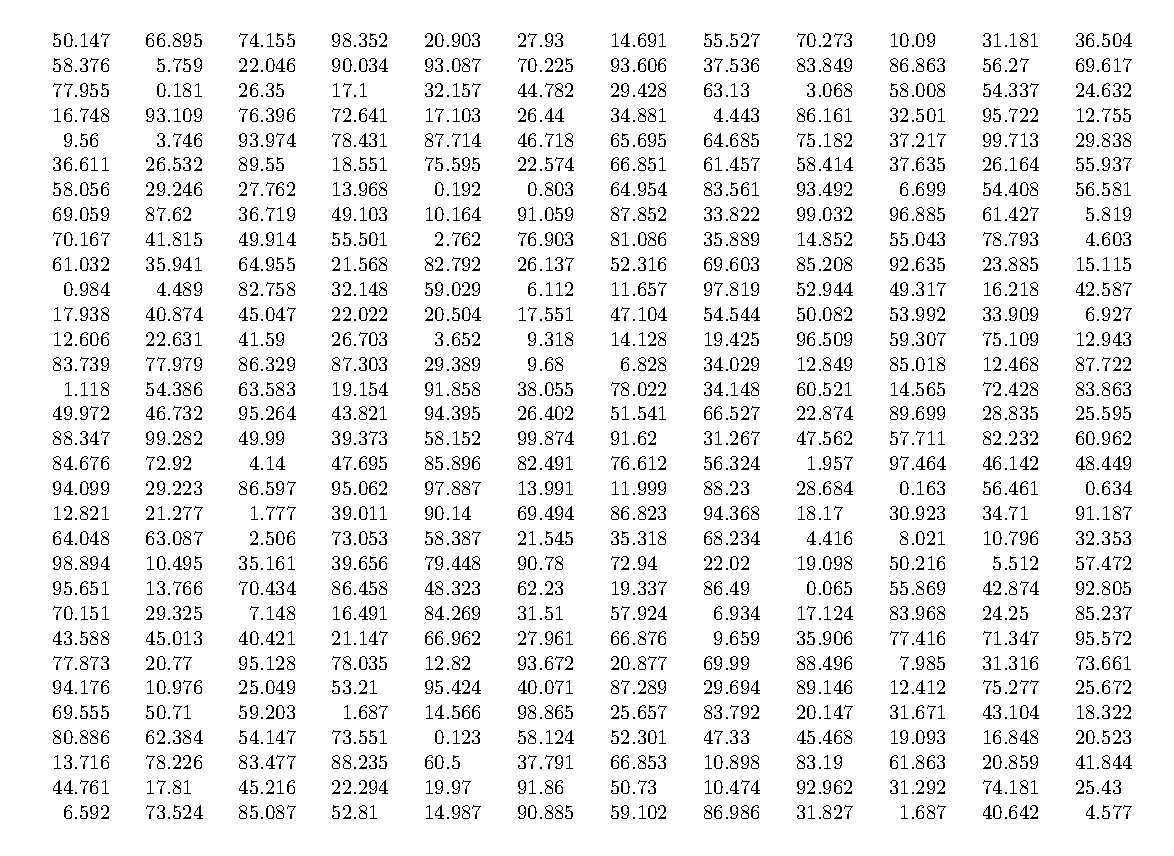
\includegraphics[width=\textwidth]{BreiteTabelle}
\end{table}


\end{document}